\documentclass[a4paper,report,headsepline]{scrreprt} 

\usepackage{xcolor} 
\usepackage{graphicx}
\usepackage[german]{babel}
\usepackage[utf8]{inputenc}
\usepackage[T1]{fontenc}
\usepackage{ae}
\usepackage{comment}


\usepackage[automark]{scrlayer-scrpage} 

% headsepline=Dicke:Länge (jeweils optional, die Dicke ist auf 0.4pt voreingestellt)
\KOMAoptions{headsepline=0.5pt} 
\addtokomafont{headsepline}{\color{black}}

\begin{document}


\title{ \begin{Huge}
\textbf{Pflichtenheft}
\end{Huge} \\ f{\"u}r das I\&K Projekt \dq Learning Spaces\dq}
\author{Anika Balke, Daniel Hartmann, Lisa Peter, \\ Maximilian Hartwich, Yuliya Karybochkin}
%\date{} %%Wenn kommentiert, wird das aktuelle Datum verwendet.

\maketitle


\tableofcontents
\clearpage



\chapter{Zielbestimmung}\label{zielbestimmung}
Das webbasierte Buchungssystem \dq Learning Spaces \dq ist für Studierende der
Fakultät WiWi konzipiert, um die zur Verfügung stehenden Selbstlernplätze
für einen bestimmten Zeitraum zu reservieren. Zudem wird dort die Belegung
und die Verfügbarkeit der Selbstlernplätze veranschaulicht und koordiniert. Im folgenden Pflichtenheft werden für die Selbstlernplätze die Synonyme \dq Räume\dq und \dq Spaces\dq verwendet.


\section{Musskriterien}\label{musskriterien}
Für die Anwendung sind folgende drei Benutzergruppen erforderlich:
\begin{itemize}
\item \textbf{Mitarbeiter \& Dozenten \& Studenten als Benutzerrolle}
\begin{itemize}
\item Über lokalen Nutzeraccount (Benutzername und Passwort) am System anmelden 
\item Raumbuchungen durchführen:
\begin{itemize}
\item Räume maximal eine Woche im Voraus buchbar 
\item Zeitslots analog der Vorlesungszeit
\item Jeder Nutzer kann maximal eine Buchung pro Woche durchführen
\item Doppelbelegungen dürfen nicht vorkommen
\end{itemize}
\item Eigene Raumbuchung anzeigen lassen und zuvor gebuchte Space stornieren.
\item Sichtbarkeit aller blockierten und freien Raumbelegungen für alle Nutzer in HTML und PDF Format
\item Dashboard zur Anzeige persönlicher bevorstehender Buchungen, sowie Anzeige zur Verfügung stehender Funktionen
\item Suchfunktion beziehungsweise Anzeigeoption freier Räume zu einem vom Benutzer auswählbaren Zeitpunkt
\item Belegung anzeigen lassen: (/LF50) Für jeden Raum bzw. Space kann sich der Benutzer die aktuelle Belegung anzeigen lassen
\end{itemize}


\item \textbf{Spaces inklusive externem Display}
\begin{itemize}
\item Installation externer Displays zur Anzeige einer Belegungsübersicht
\end{itemize}


\item \textbf{Benutzer mit erweiterten Rechten (Admin)}
\begin{itemize}
\item Verwaltung von Benutzern und Selbstlernplätzen
\item Anlegen, Editieren und Löschen von Selbstlernplätzen und Benutzern
\item Vollzugriff auf alle Funktionen und Daten
\end{itemize}
\end{itemize}

\section{Wunschkriterien}\label{wunschkriterien}
\begin{comment}
Kriterien, die optional erfüllt werden dürfen.
\end{comment}


\begin{itemize}
\item \textbf{Mitarbeiter, Dozenten und Studenten der htw saar}
\begin{itemize}
\item Login über htw saar Kennung --> LDAP Schnittstelle (ist das die Schnittstelle zur htw Datenbank??)
\item Anzeige der Ressourcen in jedem Raum (Plätze, Flipchart oder ähnliches)
\item Hilfe über Button anfragen

\end{itemize}

\item Benachrichtigungsemail bei Buchung, Stornierung
\item Erinnerungsmail kurz vor der Reservierung
\item Dozenten besitzen die Fähigkeit Buchungen zu überschreiben
\item Studenten können untereinander Räume anfragen
\item Hilfebutton zur Kontaktaufnahme bei Nachfragen und Komplikationen
\item Internationalisierung, sodass das System in englischer Sprache angezeigt und genutzt werden kann

\end{itemize}

\section{Abgrenzungskriterien}\label{abgrenzungskriterien}
%%\comment{Kriterien, die auf keinen Fall erfüllt werden dürfen.}

\begin{itemize}
\item \textbf{Mitarbeiter, Dozenten und Studenten der htw saar}
\begin{itemize}
\item Admin-Rechte 
\item Vollzugriff auf Daten und Funktionen
\item Mehrfache Raumbuchungen pro Woche 
\item Doppelbelegung eines Spaces 
\item Space für länger als einen Zeitblock buchen
\end{itemize}

\item \textbf{Spaces inklusive externer Displays}
\begin{itemize}
\item Anzeige einzelner Nutzerdaten
\item Anzeige einzelner Admin Funktionen
\end{itemize}

\end{itemize}





\chapter{Projektmanagement}\label{projektmanagement}

\renewcommand{\chapterpagestyle}{scrheadings}

Dieser Abschnitt des Pflichtenhefts definiert den groben Zeitplan sowie die Ziele der einzelnen Projektphasen. Zur Umsetzung des Projektes wurden insgesamt 100 Stunden pro Person zur Verfügung gestellt. Vor dem Beginn des Projektes wurde diese Zeit in verschiedene Phasen aufgeteilt, die während des Entwicklungsprozesses durchlaufen werden. Zunächst wurde das Projektteam zusammengestellt. Anschließend folgte nach Auswertung des Lastenheftes die Analysephase, die durch das Analysieren der Anforderungen anhand zwei Kundengesprächen gekennzeichnet ist. In Abbildung 2.1 lassen sich die Hauptprojektphasen, deren jeweiliger Abschluss ein Meilenstein des Projektes darstellt, inklusive grober Zeitplanung entnehmen. Unterteilt wurden die Projektphasen bzw. die Meilensteine zudem für einen besseren Überblick in organisatorische bzw. verwaltende Aufgaben (orange) und entwickelnde Aufgaben (blau).\\

\begin{figure}[h]
   \centering
   \caption{Zeitplan mit Meilensteinen}
   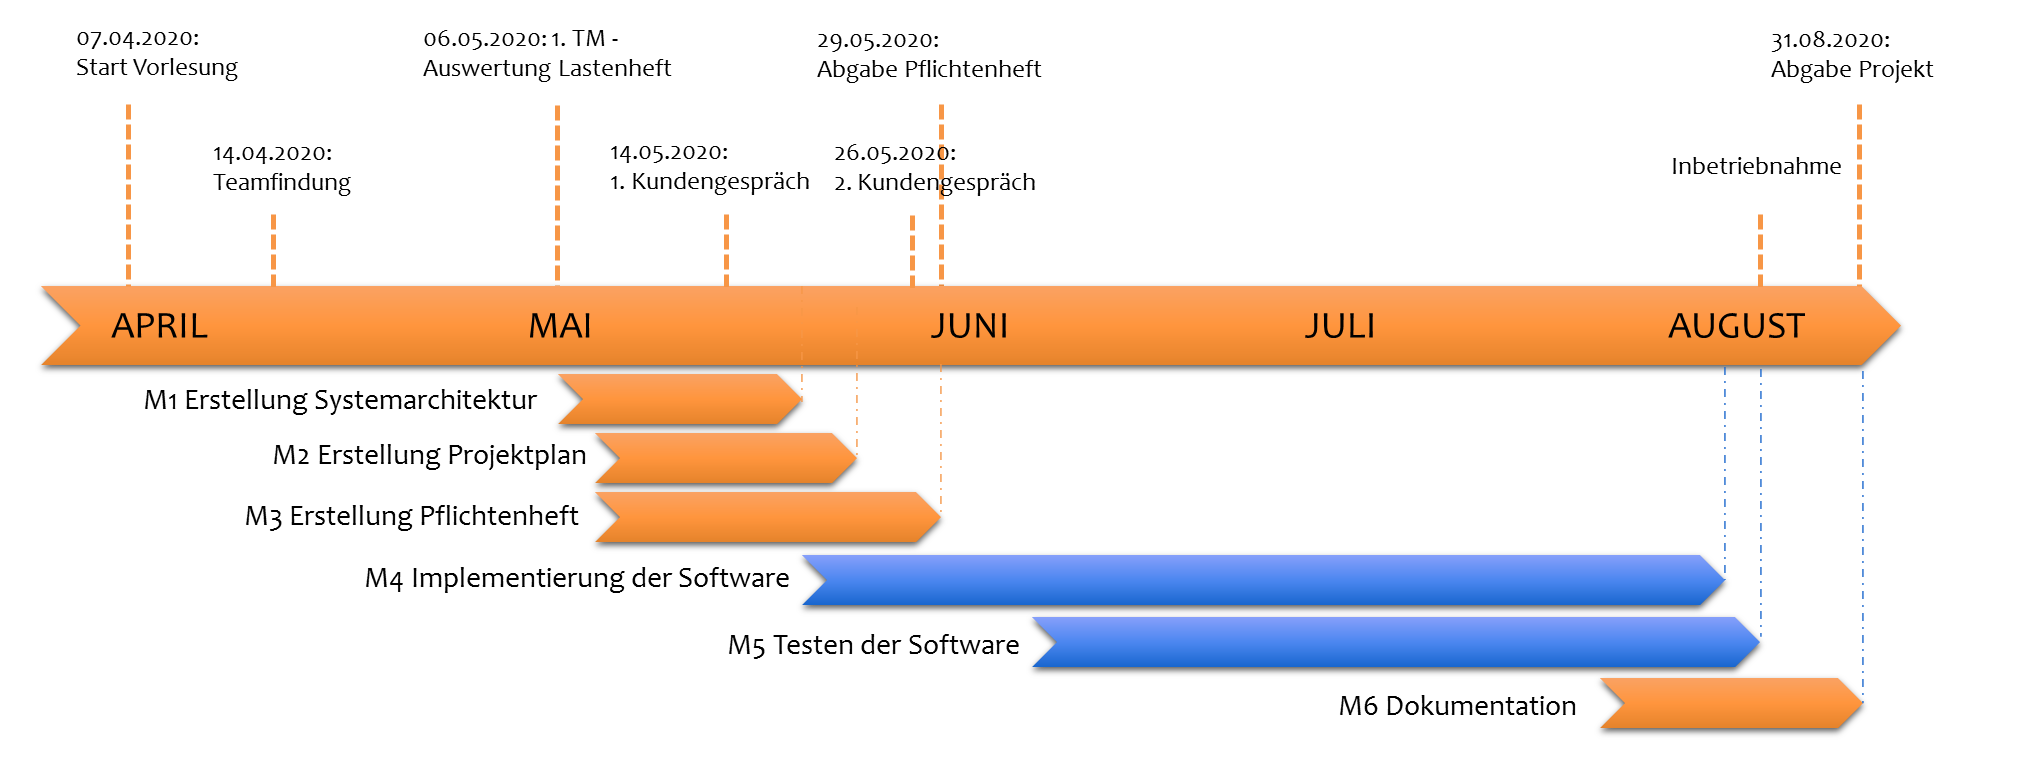
\includegraphics[width=1\textwidth]{Meilenstein}
   \label{fig:Zeitplan}
\end{figure}

\begin{itemize} 
\item M1: Erstellung der Systemarchitektur. 
In der ersten Phase wird die Systemarchitektur definiert. Hierzu zählen die Systemmerkmale, Aktivitäten, Zustände und Anwendungsfälle. Ziel dabei ist das Verschaffen eines Gesamtüberblickes. Zur visuellen Darstellung wird das Visualisierungswerkzeug „ArgoUML“ genutzt. Basierend auf diesem Systementwurf soll das Pflichtenheft erarbeitet werden. Ferner soll dies als Grundlage der zu erstellenden technischen Dokumentation dienen.

\item M2: Erstellung des Projektplans
In der zweiten Phase sollen durch den Projektmanager einzelne Aufgabenbereiche den Mitgliedern des Projektteams, anlehnend an deren Fähigkeiten, zugewiesen werden. Ferner ist ein Zeitplan inklusive Meilensteine zu definieren. Ziel hierbei ist die Festlegung des Projektumfangs.

\item M3: Erstellung des Pflichtenhefts
Bis spätestens 26.05.2020 ist das Pflichtenheft, das mit Hilfe des Textsatz-Systems „LaTeX“ erstellt wird, nach Überprüfung auf Vollständigkeit abzugeben. Darin enthalten sind die Realisierungsvorgaben samt Erläuterungen zur Umsetzung des Projektes. Ferner soll die relevante programminterne Struktur dem Kunden nahegebracht werden. Ziel davon ist die Freigabe des Entwurfs durch den Kunden.

\item M4: Implementierung der Software 
Nach erfolgreicher Freigabe kann der Entwurf realisiert werden. In dieser Phase wird mit dem Django Framework die webbasierte Anwendung „Learning Spaces“ entwickelt. Parallel dazu beginnt nach zwei Wochen die Testphase. Die gewonnenen Erkenntnisse aus der Testphase werden zur Erkennung und Behebung von Fehlern in der Software genutzt. Es werden solange die in der Testphase identifizierten Mängel behoben bis die finale Version der Anwendung, geschrieben worden ist. 

\item M5: Testen der Software
Parallel zur Implementierungsphase beginnt nach zwei Wochen die Testphase. Die Anwendung durchläuft so lange Kontrollen bis keine Mängel in Bezug auf die Qualität und Erfüllung, der für ihren Einsatz definierten Anforderungen, mehr vorzuweisen sind. Den Abschluss kennzeichnet die Inbetriebnahme der fehlerfreien Anwendung. Das Projektziel wurde  erreicht  und  das  Projekt  wurde  den Anforderungen entsprechend zur vollen Zufriedenheit des Auftraggebers umgesetzt.

\item M6: Dokumentation
Zum Schluss wird ein Projektabschlussbericht mittels des Textsatz-Systems „LaTeX“ erstellt. Dieser dient zur ausführlichen Dokumentation der erreichten Projektziele für die Projektbeteiligten und insbesondere den projektexternen Personen.  Den Abschluss dieser Phase bildet die erfolgreiche Abgabe des Projektes.



\item UML Diagramme zur Beschreibung der Software
\item Datenmodell der Anwendung

\item Wireframes

\end{itemize}

\chapter{Produkteinsatz}\label{produkteinsatz}

\section{Anwendungsbereiche}\label{anwendungsbereiche}
Grundsätzlich stellt das System eine Übersicht und Koordination über die Learning Space-Ressourcen dar.

\section{Zielgruppe}\label{zielgruppe}
Mitarbeiter, Dozenten und Studenten der htw saar.


\section{Betriebsbedingungen}\label{betriebsbedingungen}
\begin{itemize}
\item Die Anwendung soll zu jeder Tages- und Nachtzeit aufrufbar und bedienbar sein, so lange die Buchungen maximal 7 Tage vor der Nutzung gebucht werden.
\item Stornierungen jederzeit möglich.
\item DSGVO konform.
\end{itemize}


\chapter{Produktumgebung}\label{produktumgebung}
Sind verschiedene Betriebssysteme oder Datenbanken vorhanden / muss auf versch. ? zugegriffen werden?

\section{Software}\label{software}
\begin{itemize}
\item Exchange Abgleich
\item LDAP-Schnittstelle
\item sonstige API's???
\item Client: 
\begin{itemize} 
\item HTML 5.0 kompatibler Browser
\end{itemize}
\item Server:
\begin{itemize} 
\item J2SE 1.4
\item Tomcat 5.0
\item PostgreSQL 7.4
\end{itemize}

\end{itemize}

\section{Hardware}\label{hardware}
\begin{itemize}
\item Client: 
\begin{itemize} 
\item Internetfähiger Rechner
\item Smartphone???
\item Tablet???
\end{itemize}
\item Server:
\begin{itemize} 
\item Internetfähiger Rechner
\begin{itemize}
\item 'ausreichenden Plattenspeicher für Software und Datenbank'
\item 'Rechenleistung entsprechend Benutzerwahl': wie viele Nutzer hat die htw??

\end{itemize}
\end{itemize}
\end{itemize}


\section{Orgware}\label{orgware}
\begin{itemize}
\item Internetverbindung
\item Admin, der das System einrichtet und pflegt.
\end{itemize}

%%\section{Produkt-Schnittstellen}\label{produkt-schnittstellen}

\chapter{Produktfunktionen}\label{produktfunktionen}
Konkretisierung Lastenheft-Anforderung mit Verweis auf Lastenheftnummerierung.

\section{Anonymer Benutzer}
/F10/ Anzeige möglicher zu benutzender Learning Spaces
\section{Mitarbeiter, Dozenten, Studenten der htw saar als Benutzerrolle}

\subsection{Anzeige und Navigation}
\begin{itemize}
\item /F11/ Anzeige eines Learning Spaces zu einem bestimmten Zeitpunkt
\item /F12/ Anzeige der Buchungen eines Learning Spaces zu einem bestimmten 
Zeitpunkt beziehungsweise Block
\item /F13/ Anzeige von Details zu einer Buchung
\item /F14/ Anzeige persönlicher Buchungen (individueller Belegungsplan)
\item /F15/ Anzeige eines Buttons zur automatischen Kontaktaufnahme bei Nachfragen oder Komplikationen
\item /F16/ Anzeige des Systems zur Raumbuchung in englischer Sprache
\end{itemize}

\subsection{Buchung von Spaces / Räumen}
\begin{itemize}
\item /F17/ Buchung eines Spaces / Raumes zu einem bestimmten Zeitpunkt / Block
\item /F18/ Möglichkeit zur Kontaktaufnahme mit der Person, welche einen Learning Space zu einem bestimmten Zeitpunkt beziehungsweise Block gebucht hat
\item /F19/ Möglichkeit für Dozenten einen zu einem bestimmten Zeitpunkt beziehungsweise Block bereits belegten Learning Space zu überbuchen
\end{itemize}

\subsection{Stornierung von Buchungen}
\begin{itemize}
\item /F20/ Stornierung der Buchung eines Spaces / Raumes
\end{itemize}

\subsection{Personenbezogene Daten}
\begin{itemize}
\item /F21/ Änderung personenbezogener Daten durch einen Benutzer mit erweiterten Rechten (Admin) (/F26/, /F27/, /F28/) oder den Mitarbeiter, Dozenten, Studenten als Benutzerrolle selbst (/F23/)
\item /F22/ Anzeige personenbezogener Daten
\begin{itemize}
\item Benutzername
\item Passwort
\item Vorname, Nachname
\item Titel
\item E-Mail
\end{itemize}

\item /F23/ Änderung folgender personenbezogener Daten

\begin{itemize}
\item Passwort
\item E-Mail

\end{itemize}
\end{itemize}

\subsection{Anmeldung folgender personenbezogener Daten}

\begin{itemize}
\item /F24/ Login des Benutzers mit Benutzername und Passwort
\item /F25/ Logout des Benutzers
\end{itemize}

\section{Benutzer mit erweiterten Rechten (Admin)}
Einem Benutzer mit erweiterten Rechten (Admin) stehen sowohl alle zuvor aufgeführten Funktionen als auch zusätzlich noch weitere Funktionen zur Verfügung. Nach erfolgreicher Anmeldung bei dem System (/F24/) können alle diese Funktionen genutzt werden.

\begin{itemize}
\item /F26/ Anlegen von Benutzerkonten
\item /F27/ Editieren von Benutzerkonten
\item /F28/ Löschen von Benutzerkonten
\item /F29/ Anlegen der Daten zu den Spaces / Räumen
\item /F30/ Editieren der Daten zu den Spaces / Räumen
\item /F31/ Löschen der Daten zu den Spaces / Räumen
\item /F32/ Anlegen der Ressourcen der Spaces / Räumen
\item /F33/ Editieren der Ressourcen der Spaces / Räumen
\item /F34/ Löschen der Ressourcen der Spaces / Räumen

\section{Spaces}

\subsection{Anzeige}
/F35/ Anzeige der Belegung des Spaces / Raumes am jeweiligen Tag

\chapter{Produktdaten}
Beschreibung der Daten aus Benutzersicht (verbal und formal) - Diagramme.
Innerhalb des Systems zur Raumbuchung werden einige Daten persistent gespeichert.
/D10/ Benutzerdaten, alle persönliche Informationen des jeweiligen Benutzers:
\begin{itemize}
\item Benutzername
\item Passwort
\item Vorname, Nachname
\item Titel
\item E-Mail
\end{itemize}

/D11/ Belegungsdaten, alle Informationen zu den Belegungen der einzelnen Spaces / Räume

\begin{itemize}
\item Space / Raum
\item Tag und Datum
\item Uhrzeit / Block
\end{itemize}
\end{itemize}

/D12/ Daten zu den einzelnen Spaces /Räumen
\begin{itemize}
\item Bezeichnung (Nummer des Spaces / Raumes)
\item Ressource des Spaces / Raumes (z.B. PC, Tafel, Whiteboard, Beamer, …)
\end{itemize}

/D13/ Mögliche Ressourcen




\chapter{Produkt - Leistungen}\label{produkt-leistungen}

Leistungsanforderungen definieren.


/L10/ Fehlermeldung bei falscher Eingabe des Benutzernamens oder Passworts\\
/L11/ Automatische E-Mail zur Erinnerung an eine Buchung, 24 Stunden im Voraus\\
/L12/ Automatische E-Mail zur Erinnerung an die Buchung eines Learning Spaces, 24 Stunden im Voraus\\
/L13/ Automatische E-Mail zur Benachrichtigung bei erfolgreicher Stornierung der Buchung eines Learning Spaces


\chapter{Benutzeroberfläche}\label{benutzeroberfläche}
Layout des Editors, Menüführung oder Bedienung per Touch Funktion.


\begin{figure}[h]
    \centering
    \caption{Login-Layout}
    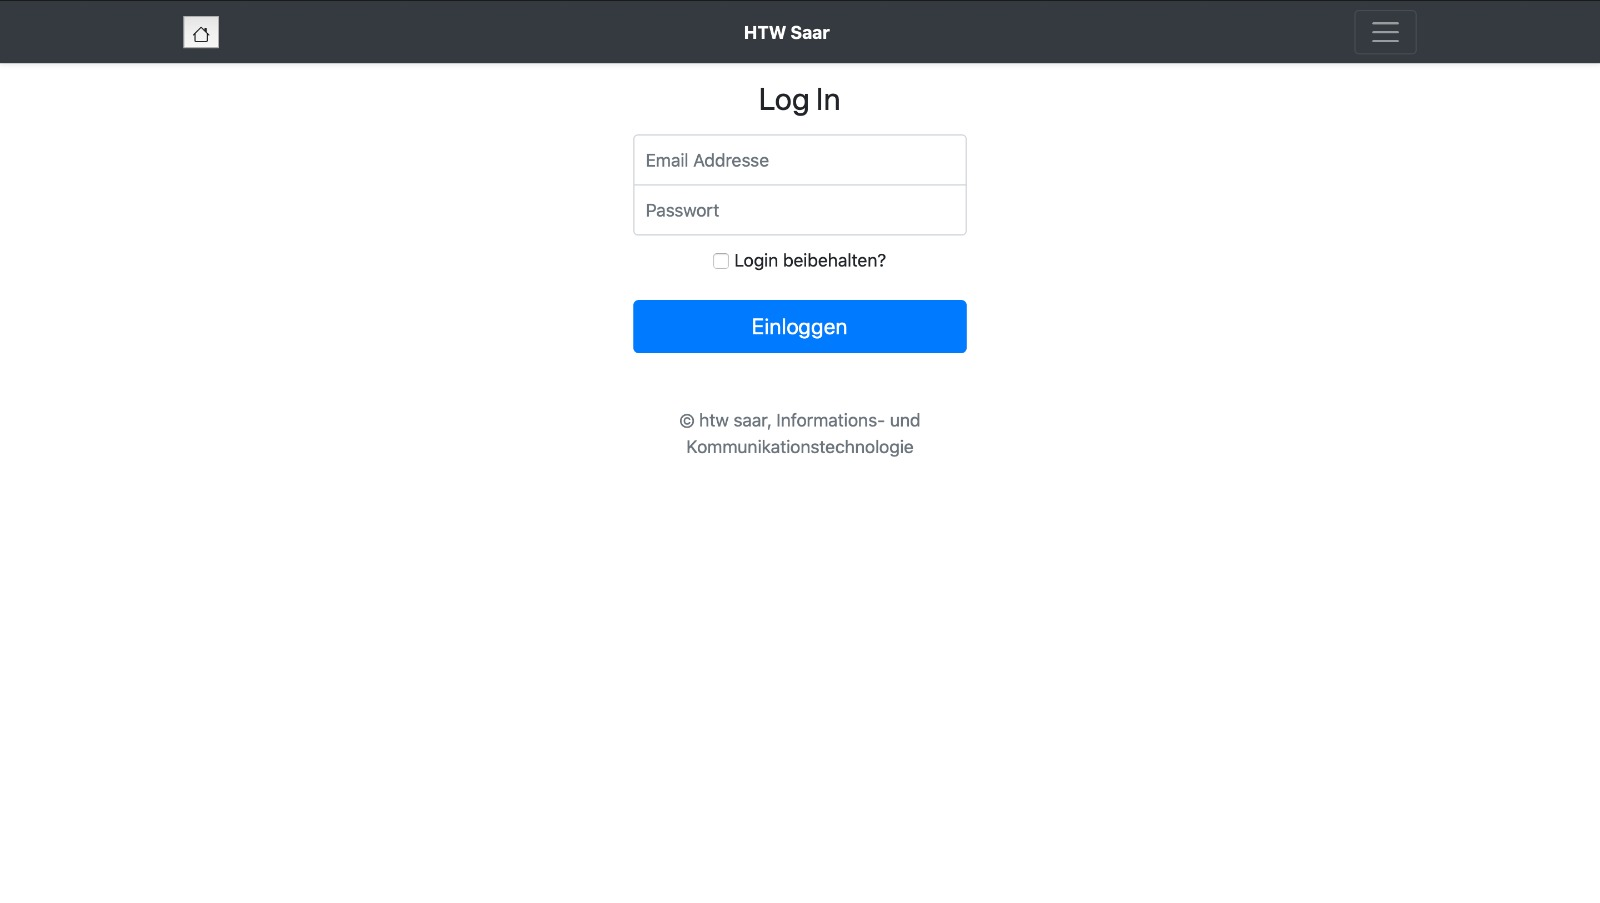
\includegraphics[width=0.7\textwidth]{Screenshot-min}
    \label{fig:login-layout}
\end{figure}

\begin{figure}[h]
    \centering
    \caption{Raumbuchungsübersicht}
    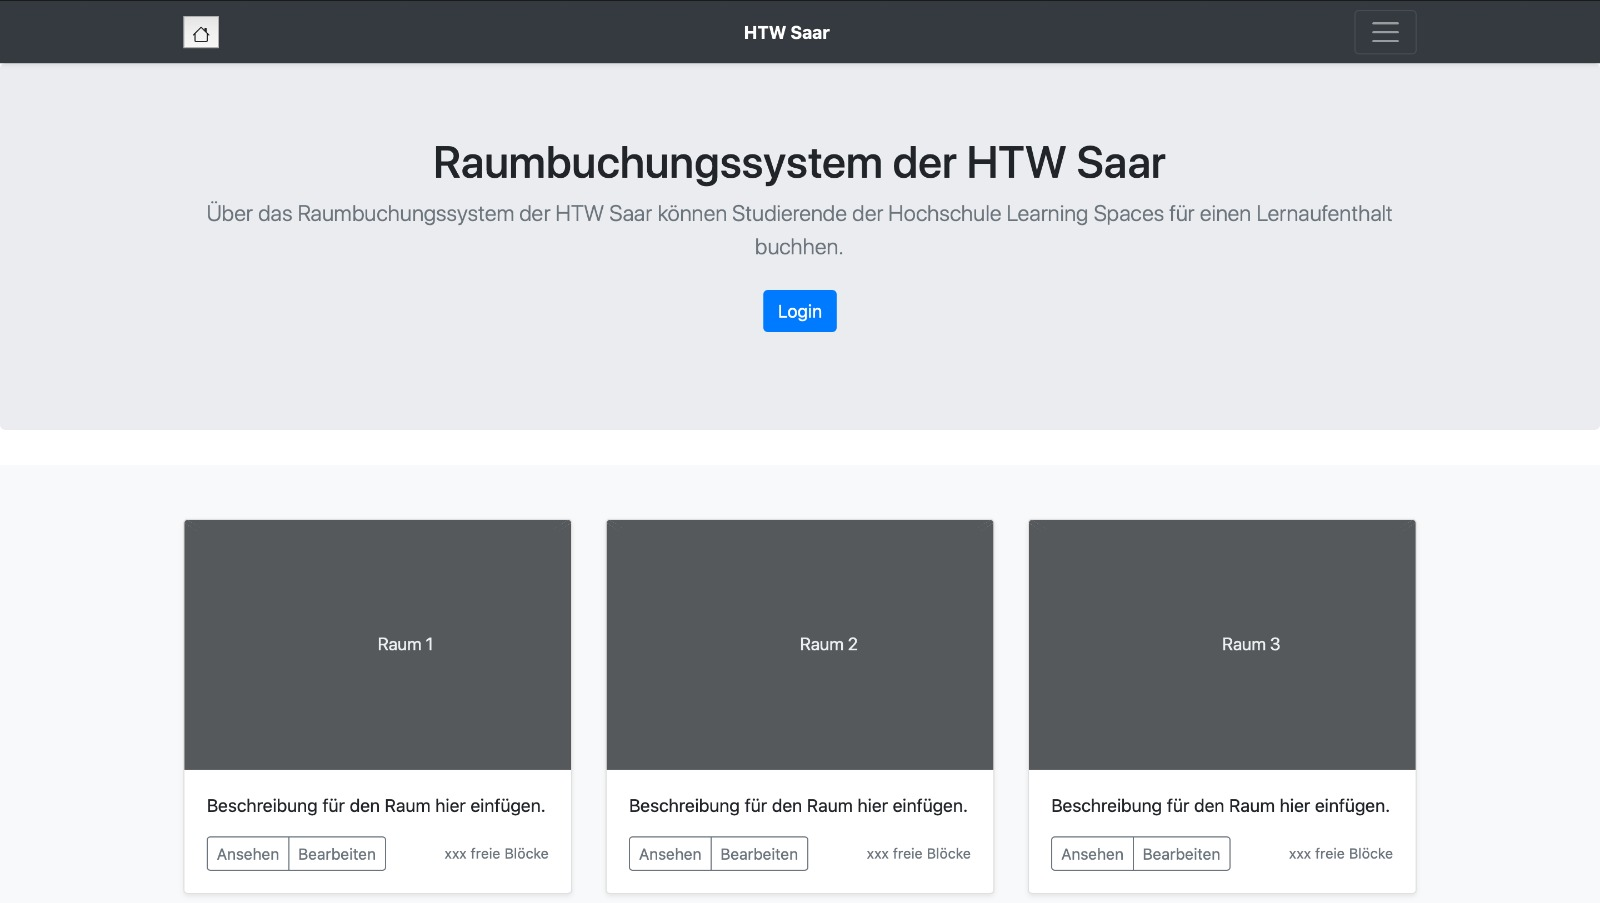
\includegraphics[width=0.7\textwidth]{Raumbuchung}
    \label{fig:raumbuchung}
\end{figure}

\begin{figure}[h]
    \centering
    \caption{Raumübersicht}
    \includegraphics[width=0.7\textwidth]{Raumübersicht}
    \label{fig:raumbuchung}
\end{figure}

\begin{figure}[h]
    \centering
    \caption{Startseite}
    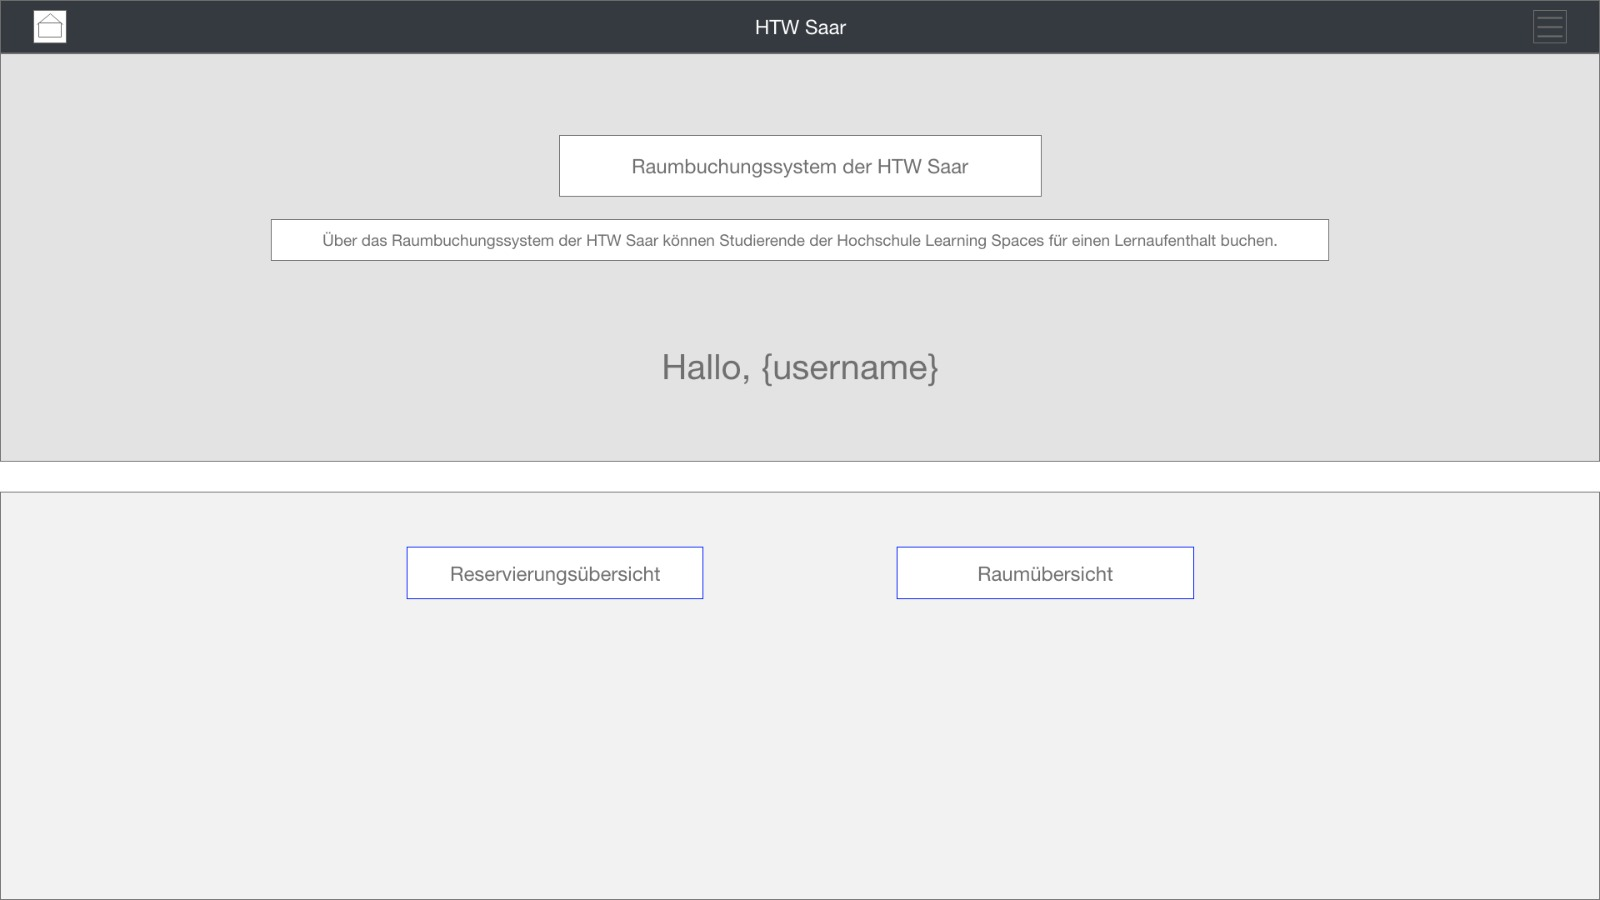
\includegraphics[width=0.7\textwidth]{Startseite}
    \label{fig:raumbuchung}
\end{figure}

\begin{figure}[h]
    \centering
    \caption{Startseite 2}
    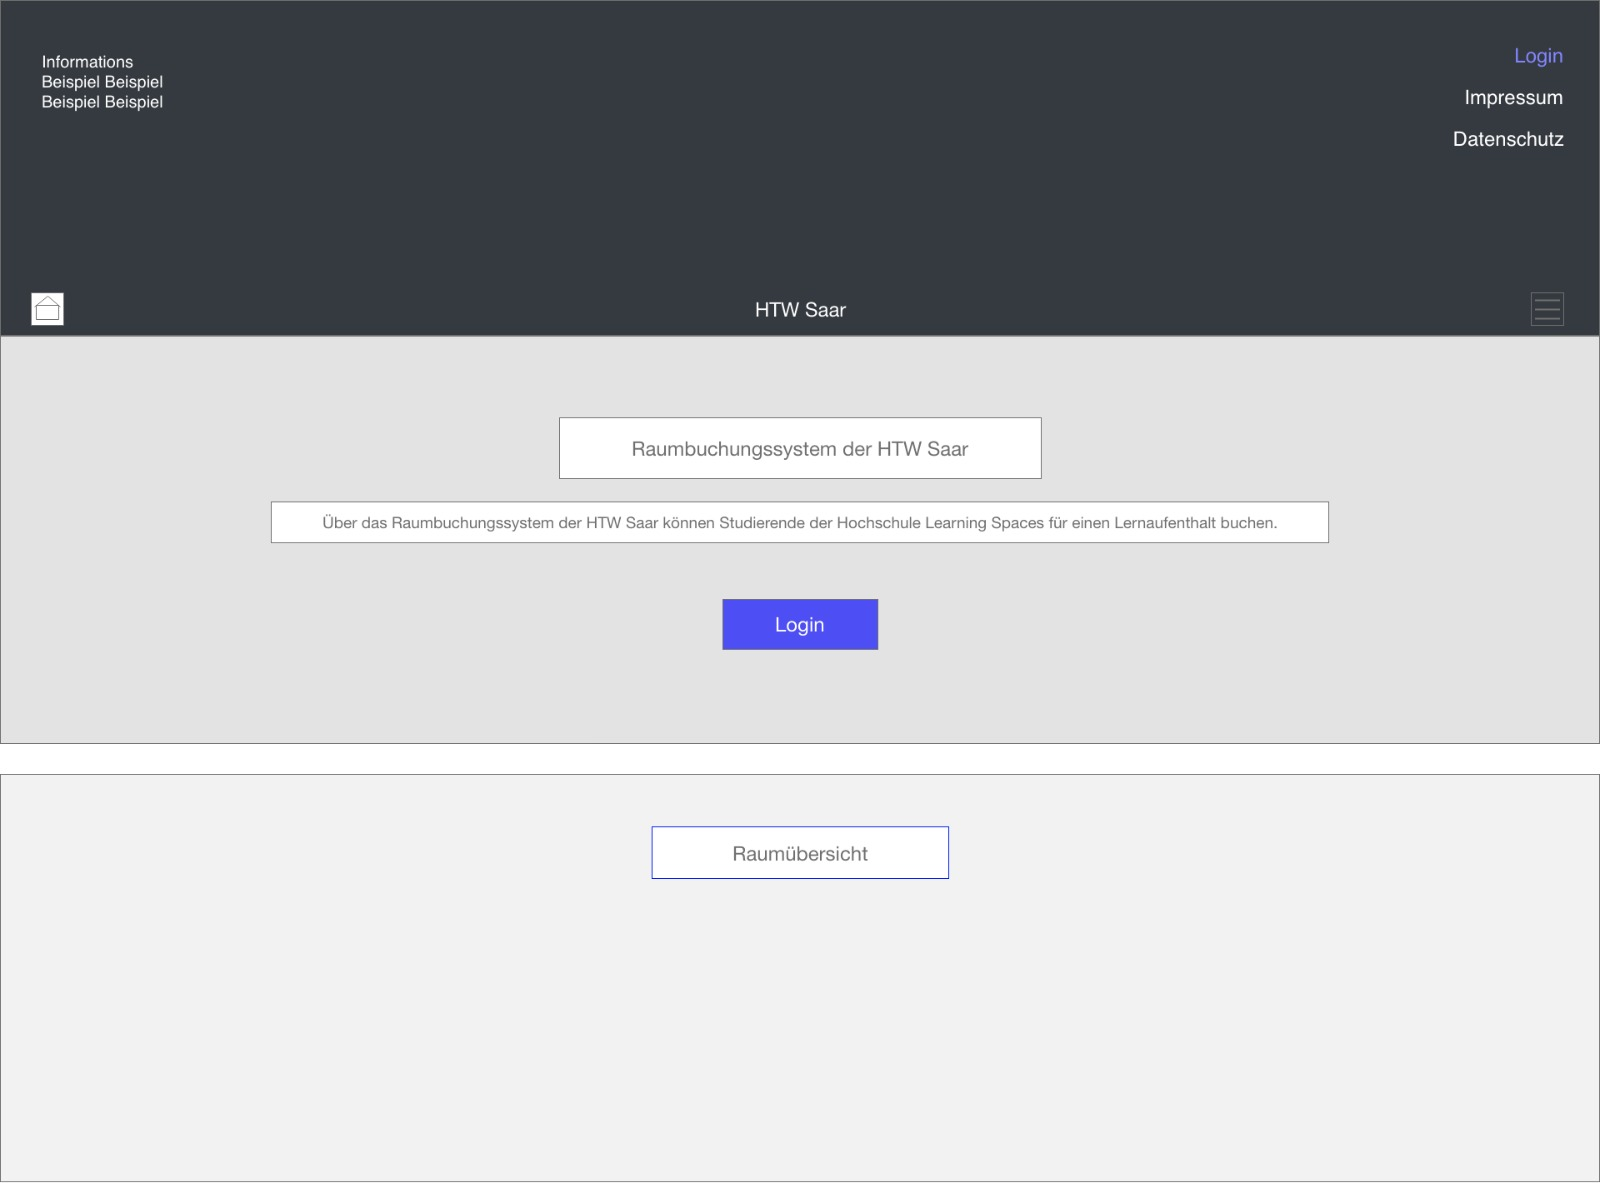
\includegraphics[width=0.7\textwidth]{Startseite 2}
    \label{fig:raumbuchung}
\end{figure}

\begin{figure}[h]
    \centering
    \caption{Startseite User}
    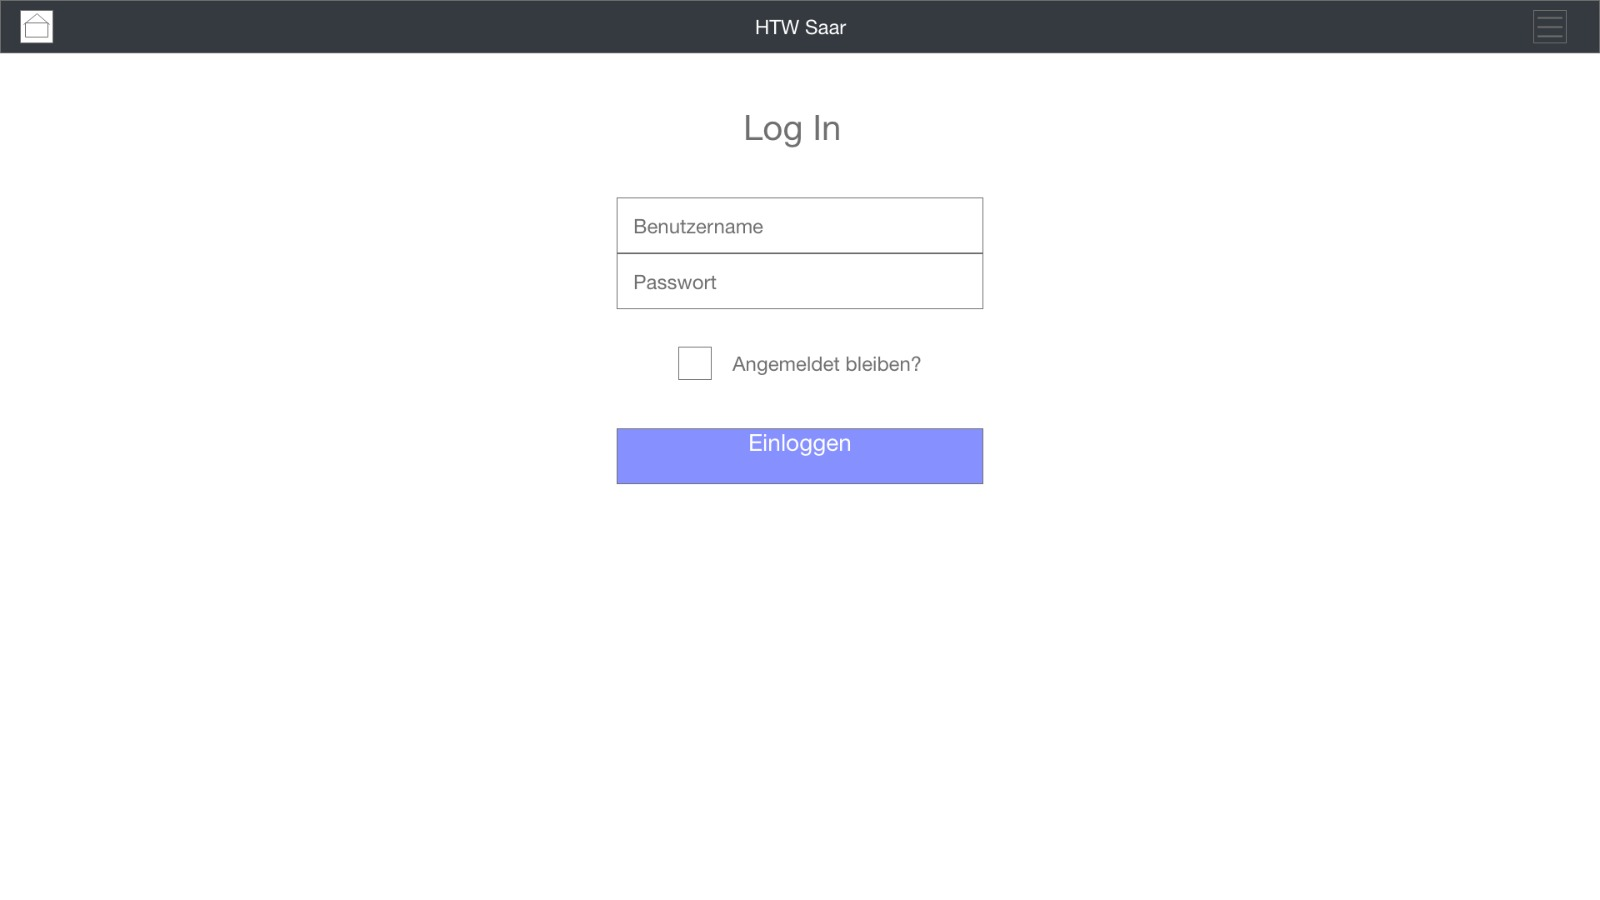
\includegraphics[width=0.7\textwidth]{Startseite User}
    \label{fig:raumbuchung}
\end{figure}

\begin{figure}[h]
    \centering
    \caption{Raumbuchungsübersicht nicht eingeloggt}
    \includegraphics[width=0.7\textwidth]{Raumbuchungsübersicht nicht eingeloggt}
    \label{fig:raumbuchung}
\end{figure}


\begin{figure}[h]
    \centering
    \caption{Raumblöcke anzeigen lassen}
    \includegraphics[width=0.7\textwidth]{Raumblöcke anzeigen lassen}
    \label{fig:raumbuchung}
\end{figure}


\begin{figure}[h]
    \centering
    \caption{Reservierungsübersicht}
    \includegraphics[width=0.7\textwidth]{Reservierungsübersicht}
    \label{fig:raumbuchung}
\end{figure}




\chapter{Qualitäts- und Zielbestimmung}\label{qualitäts-und zielbestimmung}
\begin{figure}[h]
    \centering
    \caption{Qualitäts- und Zielbestimmung}
    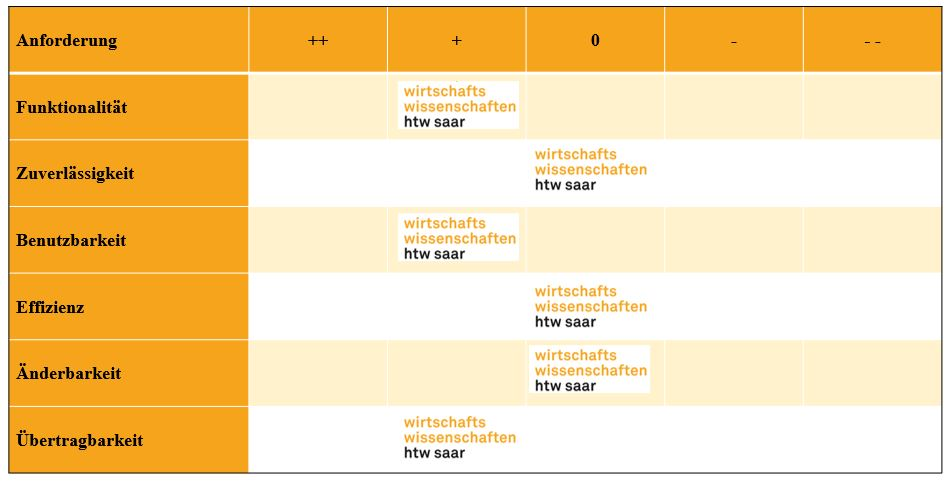
\includegraphics[width=0.7\textwidth]{Quali}
    \label{fig:qualitätsbestimmung}
\end{figure}


\chapter{Globale Testszenarien und Testfälle}\label{testszenarien}

\chapter{Entwicklungsumgebung}\label{entwicklungsumgebung}
\section{Software}\label{software}

\section{Hardware}\label{hardware}

\section{Orgware}\label{orgware}


\chapter{Ergänzungen}\label{ergänzungen}
Gesetze und Normen (DSGVO)
%%[width=16cm,height=8cm,keepaspectratio]
%%%%%%%%%%%%%%%%%%%%%%%%%%%%%%%%%%%%%%%%%%%%%%%%%%%%%%%%%%%%%
%% LITERATUR UND ANDERE VERZEICHNISSE
%%%%%%%%%%%%%%%%%%%%%%%%%%%%%%%%%%%%%%%%%%%%%%%%%%%%%%%%%%%%%
%% Ein kleiner Abstand zu den Kapiteln im Inhaltsverzeichnis (toc)
\addtocontents{toc}{\protect\vspace*{\baselineskip}}

%% Literaturverzeichnis
%% ==> Eine Datei 'literatur.bib' wird hierfür benötigt.
%% ==> Sie müssen hierfür BibTeX verwenden (Projekt | Eigenschaften... | BibTeX)
%\addcontentsline{toc}{chapter}{Literaturverzeichnis}
%\nocite{*} %Auch nicht-zitierte BibTeX-Einträge werden angezeigt.
%\bibliographystyle{alpha} %Art der Ausgabe: plain / apalike / amsalpha / ...
%\bibliography{literatur} %Eine Datei 'literatur.bib' wird hierfür benötigt.

%% Abbildungsverzeichnis
\clearpage
\addcontentsline{toc}{chapter}{Abbildungsverzeichnis}
\listoffigures

%% Tabellenverzeichnis
\clearpage
\addcontentsline{toc}{chapter}{Tabellenverzeichnis}
\listoftables

%%%%%%%%%%%%%%%%%%%%%%%%%%%%%%%%%%%%%%%%%%%%%%%%%%%%%%%%%%%%%
%% ANHÄNGE
%%%%%%%%%%%%%%%%%%%%%%%%%%%%%%%%%%%%%%%%%%%%%%%%%%%%%%%%%%%%%
\appendix
%% ==> Schreiben Sie hier Ihren Text oder fügen Sie externe Dateien ein.

%\input{Dateiname} %Eine Datei 'Dateiname.tex' wird hierfür benötigt.


\end{document}
\end{document}